\begin{figure}[h!]
    \centering
    \caption{Average rent, square footage, and rent per square foot by household 
             income decile, renters sample}
    \label{fig:ahs_rent_sqft}

    \begin{subfigure}{.69\textwidth} \centering
        \caption*{Rents per square foot}
        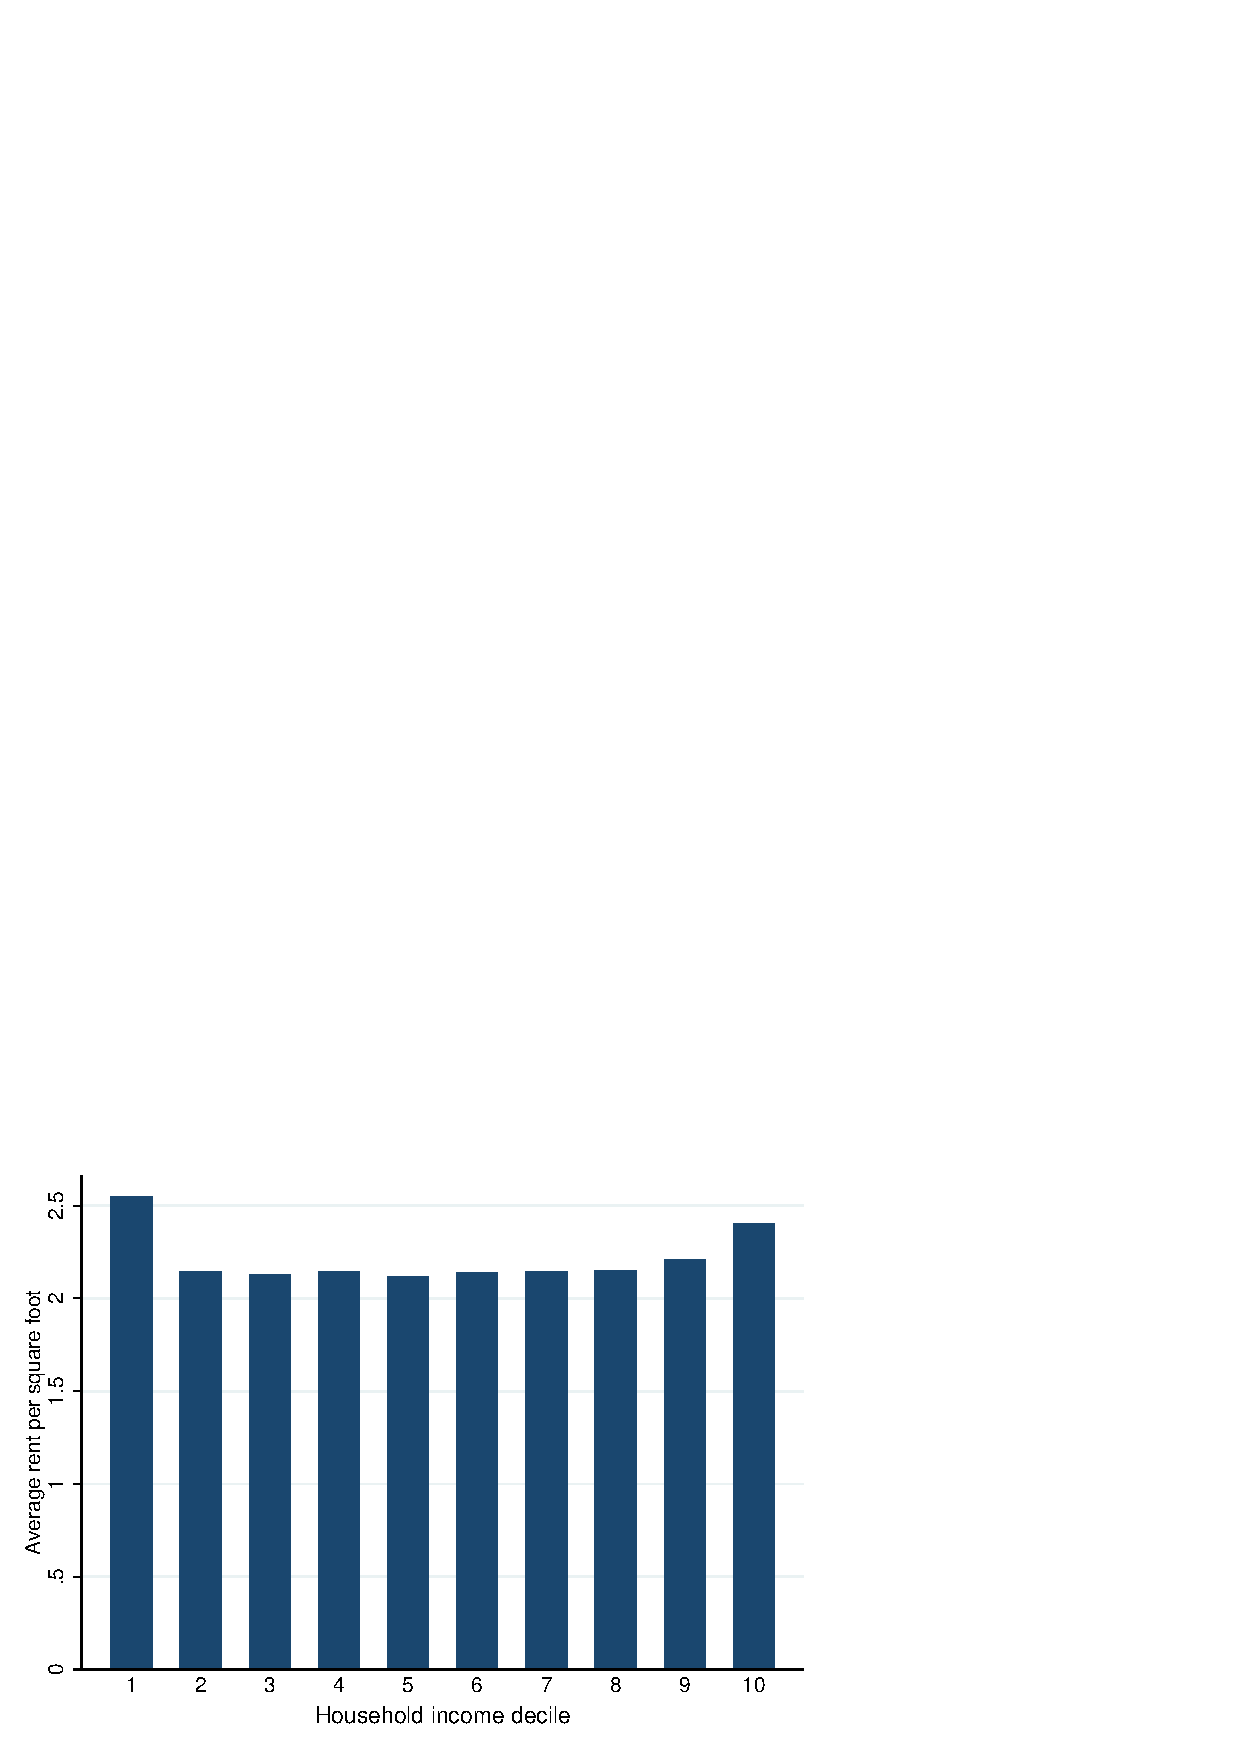
\includegraphics[width = 1\textwidth]
            {ahs/output/avg_rent_psqft}
    \end{subfigure}\\
    \begin{subfigure}{.48\textwidth} \centering
        \caption*{Rents}
        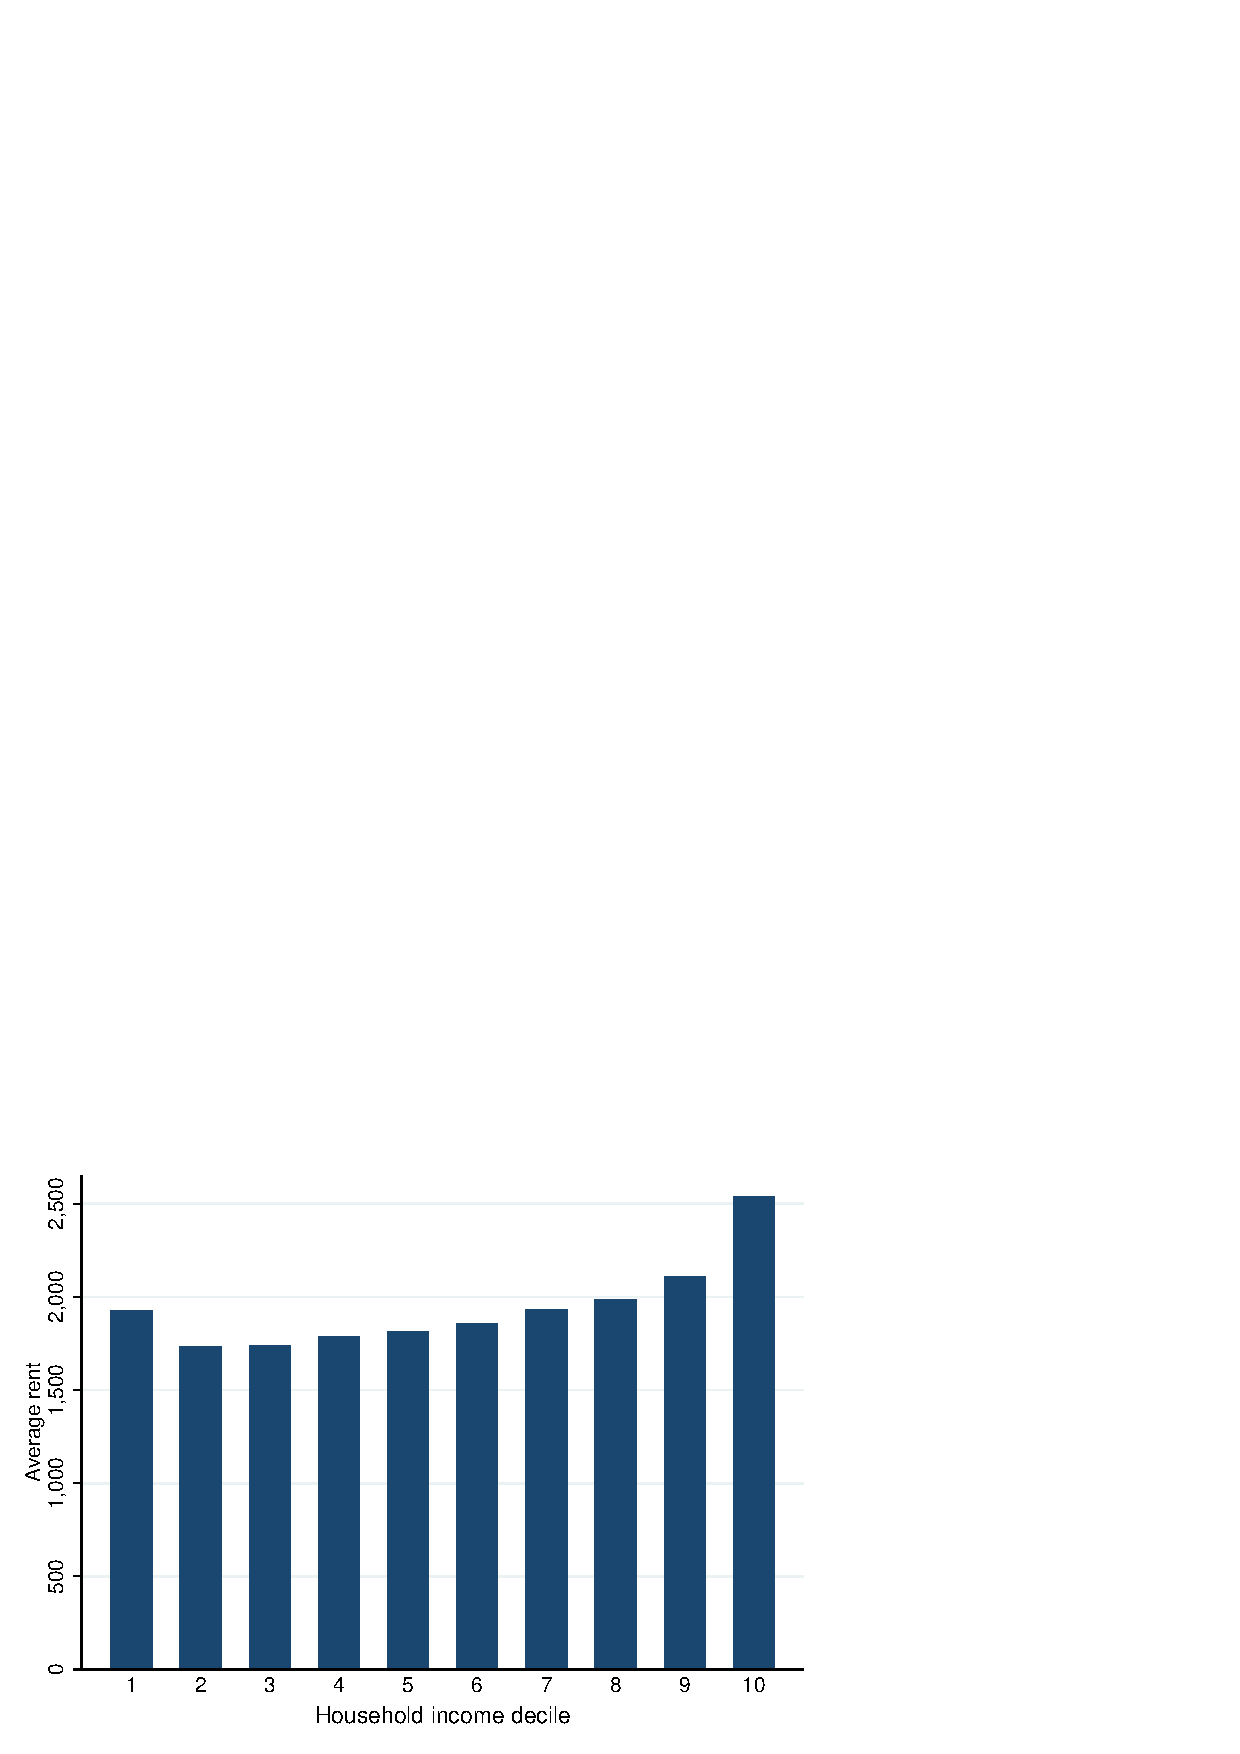
\includegraphics[width = .99\textwidth]
            {ahs/output/avg_rent}
    \end{subfigure}%
    \begin{subfigure}{.48\textwidth} \centering
        \caption*{Square footage}
        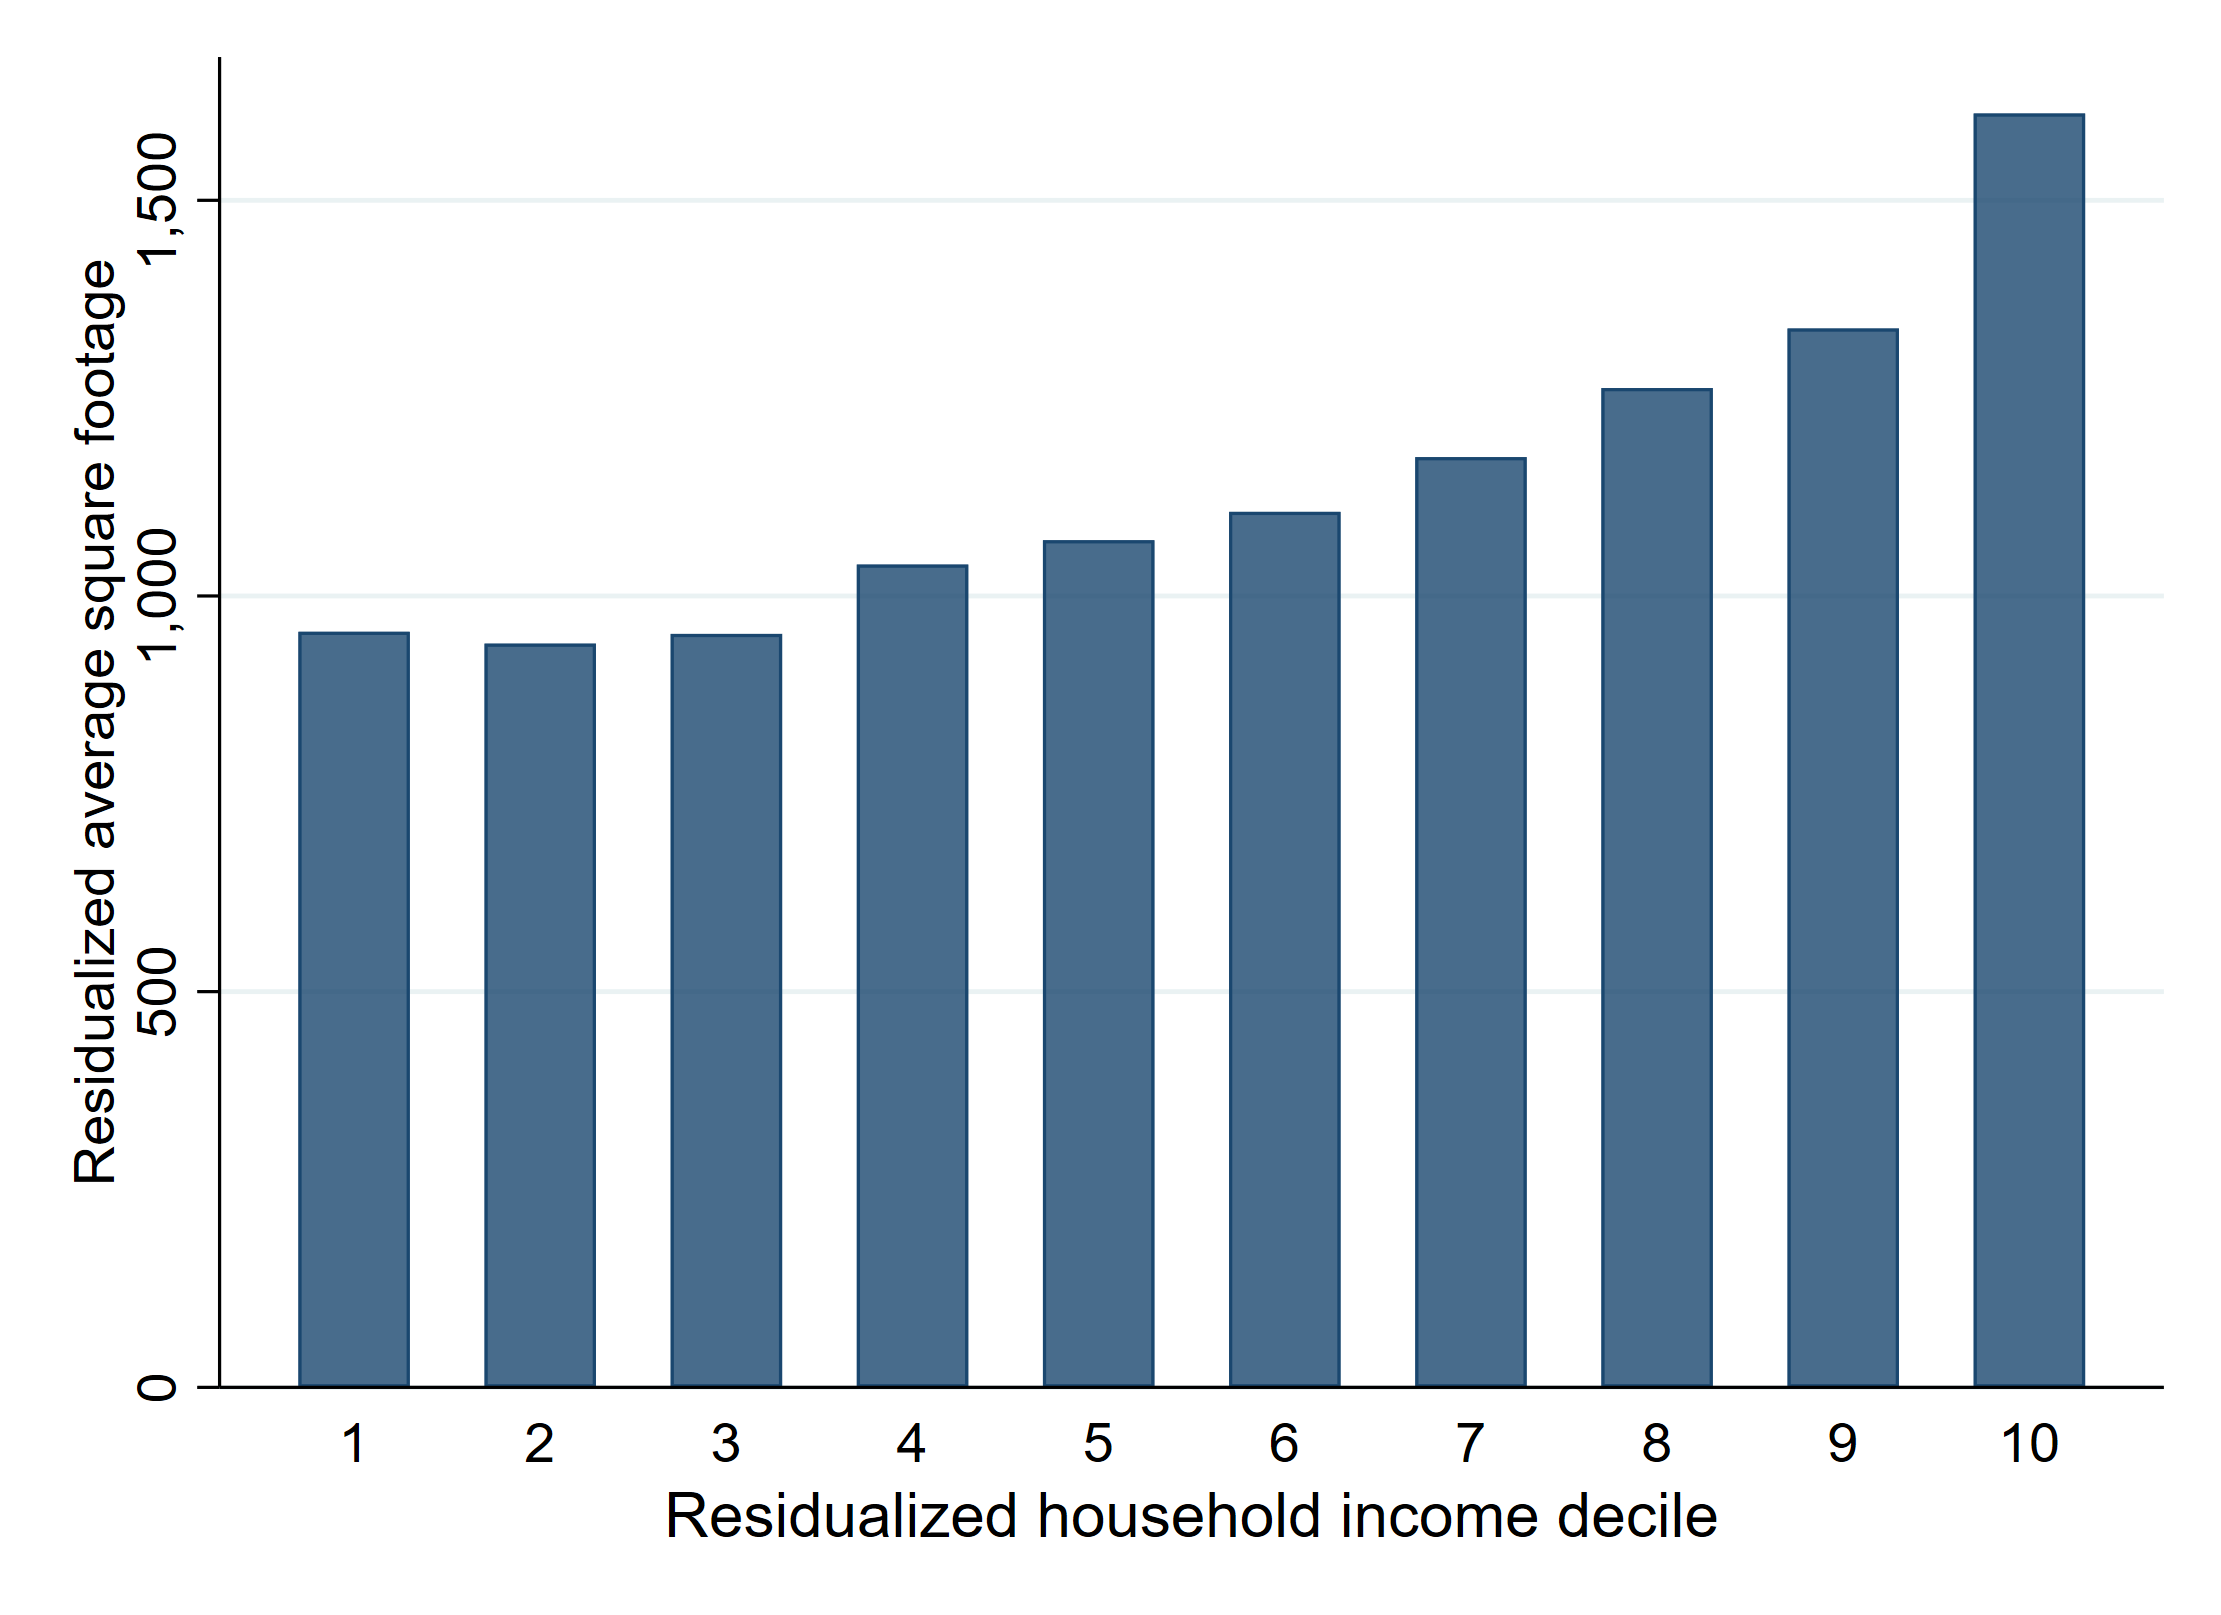
\includegraphics[width = .99\textwidth]
            {ahs/output/avg_sqft}
    \end{subfigure}

    \begin{minipage}{.95\textwidth} \footnotesize
        \vspace{3mm}
        Notes: Data are from the 2011 and 2013 American Housing Surveys.
        The top figure shows average rents per square foot by household income.
        The bottom left figure shows average rents by household income.
        The bottom right figure shows average square feet by household income.
        The variable rent per square foot is defined as total rental payments 
        divided by total square feet.
        We construct the figure as follows. 
        First, we residualize the variable in the y-axis and household income 
        by SMSA indicators, the closest analogue of CBSAs available in the data.
        Second, we construct deciles of the residualized household income 
        variable.
        Finally, we take the average of the residualized y-variable within each 
        decile.
        The sample includes households with non-missing values for square 
        footage and rental payments.
        We exclude from the calculation non-conventional housing units, such as 
        mobile homes, hotels, and others.
    \end{minipage}
\end{figure}
